\documentclass[dvipdfmx]{jsarticle}
\usepackage[T1]{fontenc}
\usepackage[dvipdfmx]{hyperref}
\usepackage{lmodern}
\usepackage{latexsym}
\usepackage{amsfonts}
\usepackage{amssymb}
\usepackage{mathtools}
\usepackage{amsthm}
\usepackage{multirow}
\usepackage{graphicx}
\usepackage{wrapfig}
\usepackage{here}
\usepackage{float}
\usepackage{ascmac}
\usepackage{url}

\title{ネットワークプログラミングを利用したアプリケーション開発}
\date{\today}
\author{日本大学 文理学部情報科学科\\5419045 高林 秀}

\begin{document}

\maketitle

\begin{abstract}
本稿は、今年度発展プログラミングの課題研究としてProcessingを用いたネットワークプログラミングを使用したアプリケーション開発を行うものである。本稿前半部では、開発の際に利用した技術やコードに関して説明を行う。本稿後半部では、実際に説明した技術を用いて、Processing上で実行可能なアプリケーションを作成する。
\end{abstract}

\tableofcontents

\section{目的}
本稿の目的は、今年度発展プログラミングの課題研究としてProcessingを用いたネットワークプログラミングを使用したアプリケーション開発を行うものである。前半部にて基本的な技術用語の説明を通して、プログラミングの際に必要な知識の復習を行う。後半部では、実際にProcessing上で実行可能なアプリケーション開発を通してネットワークプログラミングを自身のプログラムに実装する。
\section{Processingの概要}
まず、本稿の開発言語であるProcessingに関して軽く触れる。\par
Processingは、オープンソースで開発されているプログラミング言語である。主に電子アートと、グラフィック・ビジュアルデザインに特化した機能を持ち合わせており、他のプログラミング言語よりも視覚的な表現とフィードバックを簡単に得れるという特徴を持つ。\par
この言語は、米国出身のCasey Reas氏とBenjamin Fry氏によって開発・設計された。Reas氏は、マサチューセッツ工科大学のMITメディアラボの美学および計算グループの一部として、メディアアートと科学の理学修士号を取得している人物であり、Fry氏は、データの視覚化に関する専門知識を持つアメリカ人デザイナーで、カーネギーメロン大学でコンピューターサイエンスの副専攻であるコミュニケーションデザインのBFAを取得し、修士号と博士号を取得している人物である。\par
Processingの構文は、Javaに似ており、Javaをより単純化した様な構文で構成される。開発の際には、skechbookと呼ばれる統合開発環境(IDE)を利用して行う。Processingのコードとして記述された各クラスは、最終的に内部でJavaにコンパイルされ実行される。その関係上、クラス内の静的変数や静的メソッドは通常禁止で、それらを利用するには開発者が明示的に「純粋Javaモード」を指定する必要がある。\par
\begin{figure}[H]
  \centering
  
\includegraphics[scale=0.4]{images/180px-Processing_Logo_Clipped.svg.png}
  \caption{Processingロゴ}
  出典:\url{https://ja.wikipedia.org/wiki/Processing}
\end{figure}
\section{ネットワークプログラミング概要}
この章では、開発に関連する基本的な技術用語の説明を簡単に行う。
\subsection{プロトコル}
コンピュータ同士がネットワークを介して通信を行うには、データの形式や送受信の手順を定めた「プロトコル」と呼ばれるルールのようなものが必要である。プロトコルにはいくつか種類があり同一のプロトコルに従っているコンピュータ同士のみネットワーク通信を行うことが可能だ。\par
単純なアプリケーション開発でも、ネットワーク通信を行うには様々な決め事(通信先の機器の指定、データ型の指定等)を定める必要があり、異常な手間がかかる。したがって実際にネットワークプログラミングを行う際には「プロトコルスタック」と呼ばれる、プロトコルを階層化した概念が取り入れられる。この理論的モデルが「OSI参照モデル」と呼ばれるもので、それを簡略化したモデルが「TCP/IP」と呼ばれるプロトコルスタックである。
\begin{figure}[H]
  \centering
  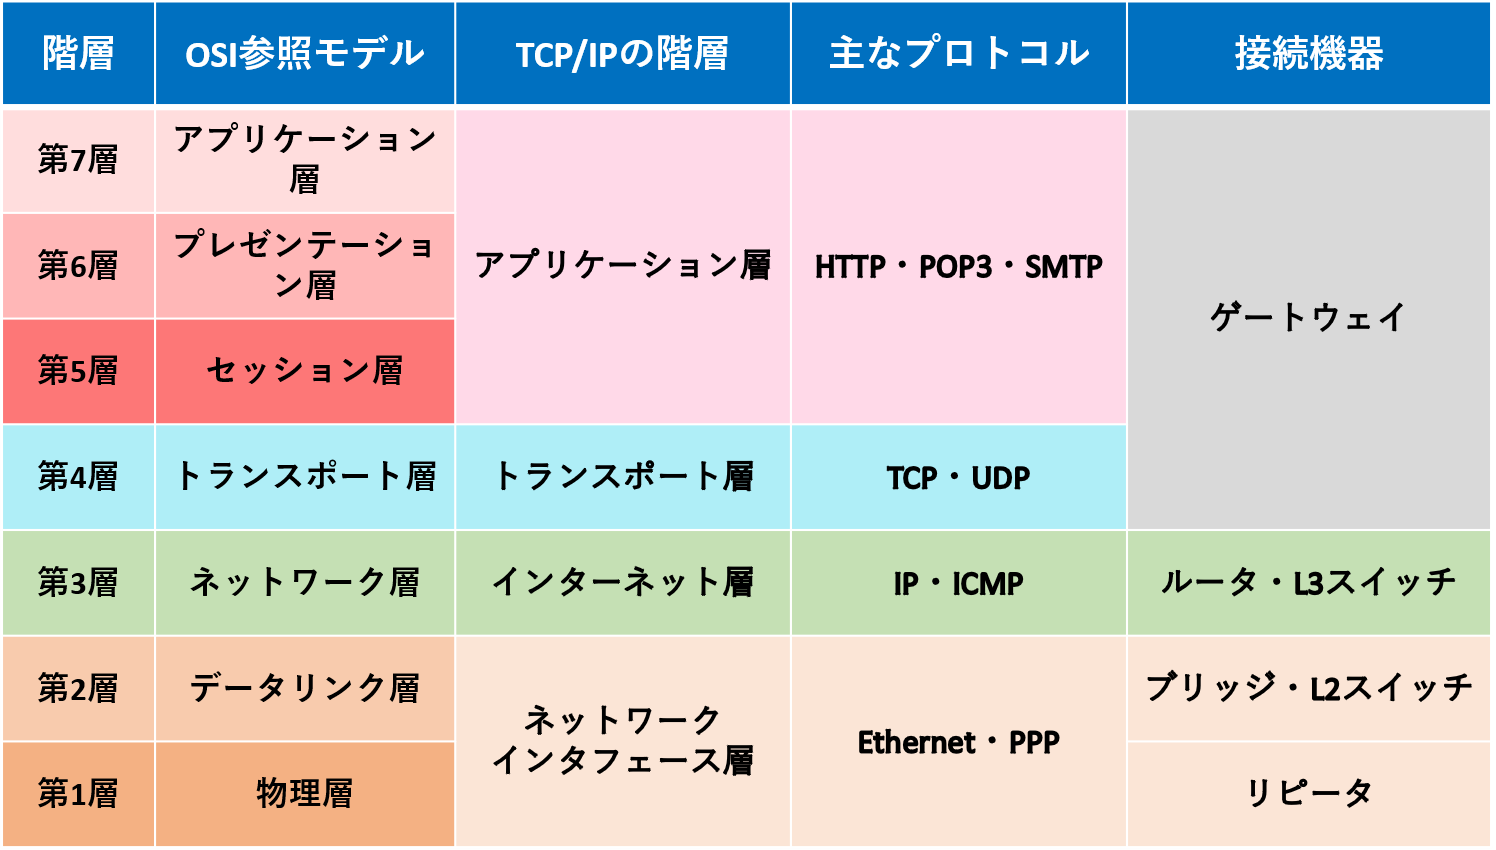
\includegraphics[scale=0.4]{images/ositcpip.png}
  \caption{OSI参照モデルとTCP/IP、その他プロトコルの関係図}
  出典:\url{https://ansl-blog.hatenablog.com/entry/2019/05/22/OSI%E5%8F%82%E7%85%A7%E3%83%A2%E3%83%87%E3%83%AB%E3%81%A8TCP%EF%BC%8FIP%E3%81%AB%E3%81%A4%E3%81%84%E3%81%A6}
\end{figure}
\subsection{TCP/IP}
TCP/IPは一般的にネットワークプロトコル群の総称を指し、接続先のコンピュータと通信を行うアプリケーションを指定するため、IPアドレスとポート番号を利用する。IPアドレスは、コンピュータの住所のようなもので、個別にコンピュータごとに割り当てられた文字列である。ポート番号は、通信を行うアプリケーションを指定する際に使用する。\par
前項の図の通り、OSI参照モデルでは細かく7層に通信機能が分類されているが、プログラミングを行う際には細かすぎるため実用的ではなかった。したがって、よりシンプルかつ実用的な階層構造にしたものがTCP/IPである。現代ののネットワーク通信ではこのTCP/IPが用いられている。
\section{クライアントサイドプログラミング}
\section{サーバーサイドプログラミング}
\section{アプリケーション実装}
\subsection{開発環境}
今回の開発は仮想マシン上で行った。下記に当時の環境を示す。
\begin{itemize}
  \item ホストOS:Window10 Home 20H2
  \item 仮想OS:Ubuntu 20.04.2 LTS
  \item CPU:Intel(R)Core(TM)i7-9700K @ 3.6GHz
  \item GPU:Nvidia Geforce RTX2070 OC @ 8GB
  \item ホストRAM:16GB
  \item 仮想RAM:4GB
  \item Processing version : 3.5.3
\end{itemize}
\subsection{制作内容}
\subsection{挙動説明}
\subsection{工夫点}
\section{巻末資料}
本稿で使用した画像、プログラムコード等はすべて以下のリンク先に掲載している。必要に応じてご覧頂きたい。
\begin{itemize}
  \item GoogleDrive:\url{}
  \item GitHub:\url{https://github.com/tsyu12345/advancedPrg/tree/master/No15-report3}
\end{itemize}



\end{document}
